\documentclass[12pt,a4paper,oneside]{report}
% ---------------- Layout & Paket Dasar ----------------
\usepackage[a4paper, top=4cm, left=3cm, right=3cm, bottom=3cm]{geometry}
\usepackage{setspace}      % untuk kontrol spasi
\usepackage{titlesec}      % untuk atur ukuran heading
\usepackage{graphicx}
\usepackage{listings}      % untuk "Daftar Tampilan" (kode/program)
\usepackage{caption}
\usepackage{fontspec}
\usepackage[backend=biber,style=ieee,sorting=nyt]{biblatex}
\usepackage{pdflscape}   % halaman landscape (auto-rotate di PDF)
\usepackage{longtable}   % tabel multi-halaman
\usepackage{booktabs}    % garis tabel yang rapi
\usepackage{multirow}    % opsional, jika ingin menggabung baris
\usepackage{array}       % untuk p{width} yang stabil
\usepackage{float}
\usepackage{plantuml} % butuh compile dengan -shell-escape
\usepackage{amsmath}
\usepackage{microtype}

\emergencystretch=2em
\addbibresource{desertasi.bib}
\setmainfont{Times New Roman} % ganti ke "TeX Gyre Termes" bila TNR tidak tersedia

% ---------------- Ukuran heading -----------------------
% Judul Bab = 14pt bold, center, dengan label BAB + angka Romawi
\titleformat{\chapter}[display]
    {\centering\bfseries\fontsize{14pt}{16pt}\selectfont}
    {BAB \Roman{chapter}}
    {0pt}
    {\vspace{1ex}}
    [\vspace{1ex}]

% Atur jarak judul bab: margin atas tetap 4cm
\titlespacing*{\chapter}{0pt}{0pt}{0.5cm}

% Subjudul (section, subsection) = 13pt bold
\titleformat{\section}
    {\bfseries\fontsize{13pt}{15pt}\selectfont}
    {\thesection}{1em}{}
\titlespacing*{\section}{0pt}{1.0\baselineskip}{1\baselineskip}

\titleformat{\subsection}
    {\bfseries\fontsize{13pt}{15pt}\selectfont}
    {\thesubsection}{1em}{}

% ---------------- Bibliografi (spasi 1) ----------------
\AtBeginBibliography{\singlespacing} % daftar pustaka spasi 1

\begin{document}
    % ===================== HALAMAN JUDUL (spasi 1) =====================
    \begin{titlepage}
        \thispagestyle{empty} % No page number
        \begin{center}
            \Large{\textbf{USULAN PENELITIAN DISERTASI}}\\[0.5cm]
            %\Large{\textbf{PENYELARASAN DATA BERBASIS RESOLUSI ENTITAS PROBABILISTIK DAN DETEKSI ANOMALI KEPATUHAN YANG TERINTEGRASI DENGAN SISTEM JAWABAN CERDAS BERBASIS PENELUSURAN}}\\[0.5cm]
            \Large{\textbf{OPTIMASI SISTEM JAWABAN CERDAS MELALUI PENYELARASAN DATA BERBASIS RESOLUSI ENTITAS PROBABILISTIK DAN DETEKSI ANOMALI KEPATUHAN}}\\[0.5cm]
            % \Large{(DATA ALIGNMENT BASED ON PROBABILISTIC ENTITY RESOLUTION AND COMPLIANCE ANOMALY DETECTION INTEGRATED WITH A RETRIEVAL-BASED INTELLIGENT QUESTION-ANSWERING SYSTEM)}\\[0.5cm]
            \Large{(Optimization of Intelligent Question-Answering Systems Through Data Alignment Based on Probabilistic Entity Resolution and Compliance Anomaly Detection)}\\[0.5cm]

            \large{\textbf{disusun dan diajukan oleh}}\\
            \large{\textbf{Benny Leonard Enrico Panggabean}}\\
            \large{\textbf{D063251008}}\\[1cm]

            
\includegraphics[width=5cm]{Logo-Resmi-Unhas-1.png}\\[0.5cm] % Replace with actual logo file

            \large{\textbf{PROGRAM STUDI DOKTOR TEKNIK INFORMATIKA}}\\
            \large{\textbf{FAKULTAS TEKNIK}}\\
            \large{\textbf{UNIVERSITAS HASANUDDIN}}\\
            \large{\textbf{MAKASSAR}}\\
            \large{\textbf{2025}}\\
        \end{center}
    \end{titlepage}
    % ===================== HALAMAN BAB 1 (spasi 1.5) =====================
    \onehalfspacing
    \chapter{PENDAHULUAN}
        \thispagestyle{empty} % No page number
        \section{Latar Belakang}
        %BEGIN-LB
        \par
            Berdasarkan data PDDIKTI yang diakses pada bulan november tahun 2025 dipropinsi sulawesi selatan terdapat tiga ratus tujuh puluh enam (376) perguruan tinggi dimana enam (6)
            diantaranya adalah institusi perguruan tinggi negeri, tiga ratus satu (301) adalah perguruan tinggi swasta, delapan belas (18) adalah perguruan tinggi kementerian lain,
            dan lima puluh satu (51) perguruan tinggi agama. Besarnya angka tersebut mencerminkan bahwa sulawesi selatan merupakan salah satu propinsi yang cukup banyak memiliki institusi pendidikan,
            institusi - institusi ini wajib melaporkan data kegiatan aktifitas akademiknya pada setiap semester, data kegiatan akademik yang dilaporkan pada setiap semester,dimana data yang dilaporkan ini
            akan menjadi acuan bagi pemerintah khususnya Kementerian Riset, Teknologi, dan Pendidikan Tinggi (Kemenristekdikti) sebagai indikator akuntabilitas dan kredibilitas perguruan tinggi terhadap pemerintah
            dan masyarakat. Kemenristekdikti melalui peraturan Menteri no 39 tahun 2025, yang mengganti Permendikbudristek Nomor 53 Tahun 2023. salah satu yang fokus pada peraturan ini adalah pemanfaatan teknologi,
            kalau sebelumnya institusi pendidikan tinggi berfokus pada pelaporan PDDIKTI sekarang perannya jauh lebih luas dimana institusi pendidikan tinggi dituntut dalam pemanfaatan teknologi pada pembelajaran,
            kurikulum hingga penjaminan mutu internal. dengan digitalisasi yang tepat , perguruan tinggi dapat lebih adaptif  dan transparan  dalam menghadapi tantangan global.
        \par
            Upaya ini juga sejalan dengan kebutuhan untuk memastikan kualitas data yang akurat mengenai staf pengajar dan kegiatan akademik, yang sangat penting untuk mendukung pembuatan kebijakan yang efektif dari tingkat unit utama hingga universitas \parencite{rizky_tito_prasetyo_155f1543}.
            Pelaporan data yang benar dan akurat merupakan kewajiban setiap perguruan tinggi, sebagaimana diatur dalam Permenristekdikti No. 61 Tahun 2016 pasal 10 butir 7 dan pasal 12 butir 3,
            serta Peraturan Menteri Pendidikan, Kebudayaan, Riset, dan Teknologi tentang Penjaminan Mutu Pendidikan Tinggi Pasal 39  \parencite[]{menteri_pendidikan_fd83efd6, i_komang_arya_ganda_wiguna_09ebc916}.
            PDDikti sendiri adalah sistem nasional yang menghimpun data pendidikan tinggi dari seluruh perguruan tinggi, di mana perguruan tinggi bertanggung jawab penuh terhadap kebenaran dan ketepatan data serta informasi yang dilaporkan secara berkala minimal satu kali setiap semester  \parencite{menteri_pendidikan_fd83efd6}.
        \par
            Sistem ini mencakup berbagai informasi vital seperti data pembelajaran, penelitian, dan pengabdian masyarakat, yang menjadi landasan bagi Kemenristekdikti dalam mengevaluasi kinerja dan akreditasi institusi  \parencite{sigit_auliana_13f309fe}  \parencite{peraturan_menteri_pendidikan_tinggi__sains__dan_teknologi_tentang_penjaminan_mutu_pendidikan_tinggi_4712741f}.
            Peraturan tersebut menggarisbawahi pentingnya akurasi data untuk akreditasi program studi dan institusi, sejalan dengan Pasal 100 PD Dikti yang mengatur perencanaan, pelaksanaan, evaluasi, dan pengembangan data oleh Kementerian  \parencite{menteri_pendidikan_fd83efd6}.
            Kementerian Riset, Teknologi, dan Pendidikan Tinggi juga mengatur standar penjaminan mutu yang baru untuk pendidikan tinggi melalui Peraturan Menteri Pendidikan Tinggi, Sains, dan Teknologi Republik Indonesia Nomor 39 Tahun 2025 yang berfokus pada peningkatan mutu penyelenggaraan pendidikan tinggi yang berdampak
            dan selaras dengan perkembangan penjaminan mutu pendidikan tinggi secara internasional  \parencite{peraturan_menteri_pendidikan_tinggi__sains__dan_teknologi_tentang_penjaminan_mutu_pendidikan_tinggi_4712741f}. Hal ini menunjukkan pergeseran fokus dari sekadar pelaporan ke arah integrasi teknologi untuk meningkatkan efisiensi, transparansi, dan akurasi dalam penjaminan mutu pendidikan tinggi  \parencite{khusnul_khotimah_8e1a714c}.
            Pergeseran ini menyoroti relevansi transformasi digital dalam pendidikan tinggi, yang bertujuan untuk meningkatkan kualitas dan aksesibilitas pembelajaran di Indonesia  \parencite{mochamad_nashrullah_00046d12}.
        \par
            Digitalisasi ini tidak hanya mempercepat komunikasi dan meningkatkan akuntabilitas, tetapi juga mendorong partisipasi publik yang lebih aktif dalam pengawasan kebijakan pendidikan  \parencite{nadiatus_soleha_f1ff679f}.
            Pentingnya akurasi dan validitas data ini juga ditegaskan oleh prinsip kehati-hatian, akurasi, dan legalitas dalam penerbitan ijazah dan sertifikat kompetensi  \parencite{peraturan_menteri_pendidikan__kebudayaan__riset__dan_teknologi_tentang_ijazah__sertifikat_kompetensi__dan_sertifikat_profesi_jenjang_pendidikan_tinggi_ee3b738b}.
            Oleh karena itu, sistem penjaminan mutu pendidikan tinggi secara sistemik harus mengevaluasi pemenuhan dan relevansi Standar Nasional Pendidikan Tinggi serta standar yang ditetapkan perguruan tinggi, mencakup bidang akademik dan non-akademik, berdasarkan PD Dikti dengan prinsip triangulasi untuk menggali kebenaran informasi  \parencite{peraturan_menteri_pendidikan_tinggi__sains__dan_teknologi_tentang_penjaminan_mutu_pendidikan_tinggi_4712741f}.
            khusus untuk perguruan tinggi swasta yang berjumlah 80\% dari total seluruh perguruan tinggi di sulawesi selatan, dimana mempunyai sumberdaya terbatas diharapkan melalui pemanfaatan teknologi khususnya teknologi informasi dan kecerdasan buatan dapat menjadi solusi alternatif untuk meningkatkan akurasi pelaporan data dan memenuhi standar penjaminan mutu yang ditetapkan pemerintah  \parencite{mochamad_nashrullah_00046d12}.
        \par
            Sebagai salah satu solusi yang ditawarkan, Kualitas data yang dilaporkan ke PDDikti sangat menentukan akuntabilitas dan kredibilitas perguruan tinggi. Data yang tidak sinkron, tidak akurat, atau tidak sesuai regulasi dapat berdampak langsung pada penilaian status akreditasi  \parencite{andi_mursidi_d2898ec2}.
            Oleh karena itu, penting untuk memastikan bahwa seluruh data yang dilaporkan memenuhi standar kualitas yang ditetapkan untuk menjaga integritas institusi dan program studi  \parencite{undang_undang_republik_indonesia_nomor_12_tahun_2012_tentang_pendidikan_tinggi_5e8158d0}.
            Faktanya, tantangan tata kelola data merupakan isu krusial di berbagai institusi pendidikan tinggi, yang dapat menghambat tercapainya kualitas data yang optimal meskipun telah ada upaya sinkronisasi  \parencite{hanim_maria_astuti_76be24e8}. Permasalahan ini sering kali diperparah oleh metode pengumpulan data manual yang lambat dan rentan terhadap inkonsistensi,
            sehingga diperlukan solusi berbasis teknologi informasi untuk mengoptimalkan manajemen akreditasi perguruan tinggi  \parencite{meuthia_rachmaniah_4adb4d40}. Integrasi kecerdasan buatan, khususnya dalam deteksi anomali kepatuhan, dapat secara signifikan meningkatkan akurasi data pelaporan PDDikti, memastikan kesesuaian dengan regulasi yang berlaku  \parencite{rani_aprillya_putri_416d128a}.
            Pemanfaatan indikator kinerja utama yang divalidasi secara sistematis sangat penting untuk mencapai akreditasi yang berkelanjutan dan untuk menunjukkan efektivitas institusional serta kualitas pendidikan secara keseluruhan  \parencite{saiful_r__mondal_e84f7350}  \parencite{yasir_javed_0c669afc}. Peningkatan kualitas data, dari entitas program studi, dosen, dan mahasiswa merupakan aspek fundamental yang mendukung transparansi, akuntabilitas,
            dan kredibilitas institusi pendidikan tinggi  \parencite{peraturan_menteri_pendidikan_tinggi__sains__dan_teknologi_tentang_penjaminan_mutu_pendidikan_tinggi_4712741f}  \parencite{rizky_tito_prasetyo_155f1543}.
        \par
            Perkembangan kecerdasan buatan (Artificial Intelligence/AI) membuka peluang signifikan untuk mengatasi tantangan tersebut. Salah satu pendekatan yang relevan adalah \textbf{probabilistic entity resolution}, yaitu teknik penyelarasan data lintas sistem yang memungkinkan identifikasi
            dan pemetaan entitas yang merujuk pada objek yang sama meskipun terdapat variasi format atau kesalahan penulisan. Melalui perhitungan probabilistik dan \textit{confidence score}, entitas mahasiswa, dosen, program studi, atau mata kuliah dapat dipadankan secara lebih akurat dibandingkan pendekatan rule-based konvensional.
            Setelah penyelarasan diperoleh, langkah penting berikutnya adalah \textbf{deteksi anomali kepatuhan}. Pendekatan hybrid—menggabungkan aturan regulasi (rule-based) dan metode machine learning seperti Isolation Forest, Local Outlier Factor, atau
            Autoencoder—dapat mendeteksi pola ketidakwajaran yang mengindikasikan potensi pelanggaran terhadap SN-Dikti maupun batasan regulatif lainnya. Temuan anomali ini menjadi komponen penting dalam audit kepatuhan akademik.
            Untuk memaksimalkan manfaat dari data yang telah selaras dan diperkaya oleh temuan anomali, penelitian ini juga mengintegrasikan hasil tersebut ke dalam \textbf{Retrieval-Augmented Generation (RAG)}. Integrasi ini memungkinkan sistem jawaban cerdas memberikan respons berbukti yang bersumber dari dokumen regulatif resmi, data ter-align antara SIAKAD–FEEDER, serta hasil analisis anomali.
            Dengan dukungan mekanisme retrieval yang relevan dan generasi jawaban yang transparan serta disertai sitasi, RAG dapat menjadi alat bantu strategis bagi pimpinan program studi dalam memahami kondisi kepatuhan akademik, melakukan evaluasi, dan mengambil keputusan yang berbasis data.
            Dengan demikian, penelitian mengenai \textbf{optimasi sistem jawaban cerdas melalui penyelarasan data berbasis resolusi entitas probabilistik dan deteksi anomali kepatuhan} memiliki urgensi akademik dan praktis yang tinggi. Penelitian ini tidak hanya menjawab permasalahan teknis sinkronisasi dan validasi data akademik,
            tetapi juga memperkuat implementasi penjaminan mutu sesuai Permendiktisaintek Nomor 39 Tahun 2025. Secara lebih luas, penelitian ini berpotensi meningkatkan kualitas tata kelola perguruan tinggi, memperkuat akuntabilitas institusi, dan mendukung upaya peningkatan kepercayaan publik terhadap pendidikan tinggi di Indonesia.
            Penelitian ini akan berkontribusi signifikan pada pengembangan kerangka kerja komprehensif untuk meningkatkan kualitas audit di sektor pendidikan tinggi, sejalan dengan kebutuhan akan transparansi dan akuntabilitas dalam pengelolaan data akademik  \parencite{sasmita_trimoelya_kau_f43471f6}  \parencite{tangguh_sang_putro_918140e5}.


        %END-LB

        \section{Rumusan Masalah}
            % start paragraf
            Berangkat dari permasalahan tata kelola data akademik yang muncul akibat ketidaksinkronan antara SIAKAD dan FEEDER PDDikti, ketidaksesuaian format data, serta munculnya anomali kepatuhan yang berdampak pada mutu pelaporan dan akreditasi perguruan tinggi,
            maka rumusan masalah dalam penelitian ini dirumuskan sebagai berikut:
            \begin{enumerate}
                \item Bagaimana karakteristik ketidaksinkronan data antara SIAKAD dan FEEDER PDDikti, serta bagaimana ketidaksinkronan tersebut memengaruhi kualitas pelaporan akademik dan kepatuhan terhadap regulasi pendidikan tinggi?
                \item Sejauh mana metode probabilistic entity resolution efektif dalam menyelaraskan data akademik lintas sistem yang memiliki variasi format, struktur, dan penulisan?
                \item Bagaimana merancang model deteksi anomali kepatuhan berbasis pendekatan hybrid (rule-based dan machine learning) untuk mengidentifikasi ketidakwajaran yang berpotensi melanggar Standar Nasional Pendidikan Tinggi (SN-Dikti)?
                \item Bagaimana mengintegrasikan hasil entity resolution dan anomaly detection ke dalam kerangka Retrieval-Augmented Generation (RAG) agar mampu menghasilkan jawaban yang akurat, berbukti, dan selaras dengan regulasi pendidikan tinggi?
                \item Bagaimana mengukur performa sistem yang dikembangkan berdasarkan metrik teknis (precision, recall, F1-score, AUC) serta metrik kualitas jawaban (faithfulness, citation precision)?
                \item Bagaimana merancang kerangka evaluasi end-to-end yang menggabungkan aspek teknis, regulatif, dan praktis untuk mendukung audit kepatuhan akademik berbasis kecerdasan buatan?
            \end{enumerate}
            
            % end paragraf
\section{Tujuan Penelitian}
        % start paragraf
        %BEGIN-TP
        Penelitian ini bertujuan untuk mengembangkan suatu model terpadu yang mampu meningkatkan kualitas tata kelola data akademik serta mendukung proses audit kepatuhan berbasis kecerdasan buatan pada perguruan tinggi. Secara khusus, tujuan penelitian ini adalah:
        \begin{enumerate}
            \item Menganalisis karakteristik ketidaksinkronan data antara Sistem Informasi Akademik (SIAKAD) dan FEEDER PDDikti untuk mengidentifikasi sumber perbedaan, inkonsistensi, serta dampaknya terhadap mutu pelaporan dan akreditasi.
            \item Mengevaluasi efektivitas metode Probabilistic Entity Resolution~(ER) dalam menyelaraskan entitas mahasiswa, dosen, program studi, dan mata kuliah pada dua sistem yang memiliki berbagai variasi format, struktur, serta standar penulisan.
            \item Merancang model deteksi anomali kepatuhan berbasis pendekatan hybrid, yaitu kombinasi aturan regulatif (rule based) dan metode machine learning (Isolation Forest, Local Outlier Factor, atau Autoencoder) untuk mengidentifikasi pelanggaran terhadap Standar Nasional Pendidikan Tinggi (SN Dikti) dan regulasi terkait.
            \item Mengintegrasikan hasil entity resolution dan anomaly detection ke dalam sistem Retrieval Augmented Generation (RAG) sehingga sistem mampu memberikan jawaban tanya jawab akademik yang akurat, berbukti, konsisten, dan dapat dipertanggungjawabkan.
            \item Mengukur performa sistem yang dikembangkan menggunakan metrik teknis seperti precision, recall, F1 score, AUC (Area Under Curve), serta metrik kualitas jawaban RAG seperti faithfulness dan citation precision.
            \item Mengembangkan kerangka evaluasi end to end yang mengintegrasikan aspek teknis, regulatif, dan praktis untuk mendukung audit kepatuhan akademik berbasis kecerdasan buatan sesuai Permendiktisaintek Nomor 39 Tahun 2025.
        \end{enumerate}
        %END-TP
        % end paragraf
        \section{Batasan Masalah}
            Agar penelitian ini terarah dan fokus, maka ruang lingkup penelitian dibatasi pada hal-hal berikut:
            % start paragraf
            %BEGIN-BM
            Untuk menjaga penelitian tetap terarah, terukur, dan sesuai ruang lingkup yang dapat diselesaikan dalam satu disertasi, penelitian ini dibatasi pada aspek-aspek berikut:
            \begin{enumerate}
                \item Ruang lingkup data terbatas pada data akademik yang dilaporkan perguruan tinggi ke PDDikti melalui SIAKAD dan FEEDER.
                \item Fokus penyelarasan data hanya menggunakan pendekatan Probabilistic Entity Resolution (ER) dan tidak mencakup metode ER berbasis deep learning yang lebih kompleks.
                \item Model deteksi anomali kepatuhan hanya mencakup kombinasi metode rule-based dan machine learning (Isolation Forest, Local Outlier Factor, Autoencoder) serta tidak mencakup eksplorasi model deteksi anomali berbasis deep generative models.
                \item Integrasi Retrieval-Augmented Generation (RAG) dibatasi pada pengambilan informasi dari regulasi resmi, data hasil entity resolution, serta temuan anomaly detection.
                \item Evaluasi sistem difokuskan pada konteks perguruan tinggi di Provinsi Sulawesi Selatan dan tidak membahas perluasan skala nasional.
                \item Aspek regulatif merujuk pada regulasi yang berlaku hingga tahun 2025, terutama Permendiktisaintek Nomor 39 Tahun 2025 dan regulasi terkait PDDikti.
            \end{enumerate}
            %END-BM
            % end paragraf
        \section{Manfaat Penelitian}
            % start paragraf
            %BEGIN-MP
            Penelitian ini diharapkan memberikan beberapa manfaat penting baik dari sisi akademik, praktis, maupun kebijakan, yaitu sebagai berikut:
            \begin{enumerate}
                \item Manfaat Akademik: Memberikan kontribusi ilmiah melalui integrasi pendekatan Probabilistic Entity Resolution, deteksi anomali kepatuhan berbasis machine learning, dan Retrieval-Augmented Generation (RAG) dalam konteks tata kelola pendidikan tinggi. Penelitian ini dapat memperkaya literatur mengenai pemanfaatan kecerdasan buatan pada audit kepatuhan akademik.
                \item Manfaat Praktis: Menyediakan model dan prototipe sistem yang dapat membantu perguruan tinggi meningkatkan akurasi dan konsistensi pelaporan data ke PDDikti, mengurangi potensi kesalahan manusia, serta mempercepat proses identifikasi masalah kepatuhan.
                \item Manfaat Teknologis: Menghasilkan kerangka kerja teknologi yang dapat diimplementasikan dalam sistem akademik perguruan tinggi untuk mendukung automasi pemeriksaan data, analisis anomali, dan penyediaan jawaban berbukti melalui RAG, sehingga meningkatkan efisiensi pengelolaan data akademik.
                \item Manfaat Kebijakan: Menjadi dasar rekomendasi bagi pemangku kepentingan pendidikan tinggi dalam merumuskan kebijakan peningkatan tata kelola data dan penjaminan mutu internal yang selaras dengan Permendiktisaintek Nomor 39 Tahun 2025.
                \item Manfaat Sosial-Institusional: Meningkatkan transparansi, akuntabilitas, dan kepercayaan publik terhadap perguruan tinggi melalui penyediaan data yang lebih akurat, valid, serta dapat dipertanggungjawabkan dalam proses akreditasi dan evaluasi kelembagaan.
            \end{enumerate}
            %END-MP
            % end paragraf
    % ===================== HALAMAN BAB 2 (spasi 1.5) =====================
    \onehalfspacing
    \chapter{TINJAUAN PUSTAKA}
    \thispagestyle{empty}
        %BEGIN-BAB2
        \section{Feeder DIKTI}
        Feeder DIKTI merupakan sistem pelaporan data perguruan tinggi yang terintegrasi dengan Pangkalan Data Pendidikan Tinggi dan menjadi infrastruktur krusial dalam manajemen akademik nasional  \parencite{international_journal_of_evaluation_and_research_in_education__ijere__f1437b0d}.
        Sistem ini dirancang untuk memastikan bahwa seluruh data penyelenggaraan pendidikan tinggi di Indonesia terkumpul secara nasional dan dapat diakses oleh berbagai pihak berkepentingan, termasuk lembaga akreditasi, pemerintah, dan masyarakat  \parencite{ngatmari_ngatmari_87a9f833}  \parencite{peraturan_menteri_pendidikan_tinggi__sains__dan_teknologi_tentang_penjaminan_mutu_pendidikan_tinggi_4712741f}.
        Data yang dikelola dalam Feeder DIKTI mencakup informasi vital seperti profil mahasiswa, riwayat studi, data dosen, kurikulum, hingga fasilitas pendidikan, yang semuanya berfungsi sebagai basis evaluasi kinerja dan penyusunan kebijakan pendidikan  \parencite{ariana_yunita_b139140c}.
        Kualitas dan keakuratan data dalam Feeder DIKTI sangat esensial karena menjadi fondasi bagi proses akreditasi institusi, evaluasi program studi, serta penentuan peringkat perguruan tinggi, sehingga ketidakakuratan dapat berdampak signifikan pada reputasi dan operasional pendidikan tinggi.
        Pengolahan data ini dilakukan melalui antarmuka aplikasi PDDIKTI FEEDER, yang kemudian disinkronkan dengan basis data Pusdatin Kemristekdikti  \parencite{ngatmari_ngatmari_87a9f833}. Penggunaan sistem ini bertujuan untuk standarisasi dan integrasi data pendidikan tinggi secara nasional, sejalan dengan kebutuhan akreditasi dan penjaminan mutu eksternal  \parencite{menteri_pendidikan_fd83efd6}.
        Pangkalan Data Pendidikan Tinggi sendiri merupakan kumpulan data penyelenggaraan pendidikan tinggi yang terintegrasi secara nasional, berfungsi sebagai sumber informasi penting bagi lembaga akreditasi, pemerintah, dan masyarakat untuk evaluasi kinerja program studi dan perguruan tinggi  \parencite{undang_undang_republik_indonesia_nomor_12_tahun_2012_tentang_pendidikan_tinggi_5e8158d0}.
        Penyampaian laporan penyelenggaraan pendidikan tinggi ke PDDikti ini wajib dilakukan secara berkala setiap semester, baik semester ganjil, genap, maupun semester antara  \parencite{muhadi_hariyanto_3071c01e}. 

        \section{Pangkalan Data Perguruan Tinggi}
        PDDikti adalah pusat data yang dikelola oleh Kementerian Riset, Teknologi, dan Pendidikan Tinggi, yang berfungsi sebagai repositori terpusat untuk seluruh data akademik dan non-akademik dari institusi pendidikan tinggi di Indonesia  \parencite{ngatmari_ngatmari_87a9f833}.
        Pangkalan data ini berperan vital dalam sistem penjaminan mutu eksternal melalui proses akreditasi, serta menjadi sumber informasi utama bagi pemerintah untuk pengaturan, perencanaan, dan pengawasan pendidikan tinggi  \parencite{menteri_pendidikan_fd83efd6}  \parencite{undang_undang_republik_indonesia_nomor_12_tahun_2012_tentang_pendidikan_tinggi_5e8158d0}.
        Setiap perguruan tinggi diwajibkan untuk melaporkan seluruh kegiatan akademik semesterannya melalui sistem Pangkalan Data Pendidikan Tinggi atau yang dahulunya dikenal sebagai Evaluasi Program Studi Berdasarkan Evaluasi Diri  \parencite{widarta_widarta_0071f08c}.
        Peraturan Menteri Riset, Teknologi dan Pendidikan Tinggi Nomor 61 Tahun 2016 secara spesifik mengatur Pangkalan Data Pendidikan Tinggi, termasuk penggunaan PDDikti Feeder sebagai perangkat lunak wajib di setiap Perguruan Tinggi untuk pelaporan penyelenggaraan pendidikan tinggi  \parencite{muhadi_hariyanto_3071c01e}.
        Data dan informasi yang termuat dalam PDDikti ini dikembangkan secara berkelanjutan oleh Kementerian untuk memenuhi kebutuhan penjaminan mutu pendidikan tinggi, dengan perguruan tinggi bertanggung jawab penuh atas kebenaran dan ketepatan data yang dilaporkan  \parencite{peraturan_menteri_pendidikan_tinggi__sains__dan_teknologi_tentang_penjaminan_mutu_pendidikan_tinggi_4712741f}.
        Oleh karena itu, sistem ini sangat kritikal bagi pengelolaan data penyelenggaraan pendidikan tinggi di seluruh Indonesia, memastikan integrasi nasional dan transparansi informasi akademik yang akuntabel  \parencite{widarta_widarta_0071f08c}  \parencite{peraturan_menteri_pendidikan_tinggi__sains__dan_teknologi_tentang_penjaminan_mutu_pendidikan_tinggi_4712741f}.
        PDDikti berfungsi sebagai sumber informasi krusial bagi lembaga akreditasi, pemerintah, dan masyarakat untuk memantau kinerja program studi dan perguruan tinggi  \parencite{undang_undang_republik_indonesia_nomor_12_tahun_2012_tentang_pendidikan_tinggi_5e8158d0}.
        Pengelolaan dan pengembangan PDDikti merupakan tanggung jawab Kementerian, atau lembaga yang ditunjuk oleh Kementerian, untuk memastikan kelengkapan dan keandalan data dalam mendukung berbagai fungsi strategis pendidikan tinggi nasional  \parencite{undang_undang_republik_indonesia_nomor_12_tahun_2012_tentang_pendidikan_tinggi_5e8158d0}  \parencite{peraturan_menteri_pendidikan_tinggi__sains__dan_teknologi_tentang_penjaminan_mutu_pendidikan_tinggi_4712741f}.
        Data yang dikirimkan ke PDDikti mencakup aktivitas mengajar dosen, perkuliahan mahasiswa, data mata kuliah, kurikulum, dan data akademik lainnya, yang menjadi indikator validitas profil seorang mahasiswa  \parencite{adi_wirawan_ef077ca7}. 


        \section{Probabilistic Entity Resolution}
        Entity Resolution (ER) adalah proses memetakan entitas yang berbeda namun merepresentasikan objek yang sama. Pendekatan probabilistik memungkinkan penyelarasan data dengan mempertimbangkan variasi penulisan dan ketidakkonsistenan format melalui perhitungan skor kemiripan dan confidence level.


        \section{Deteksi Anomali Kepatuhan}
        Deteksi anomali digunakan untuk mengidentifikasi pola data yang tidak wajar. Dalam konteks kepatuhan akademik, hal ini meliputi beban SKS dosen melebihi batas, mahasiswa dengan masa studi tidak wajar, dan ketidaksesuaian lainnya. Metode hybrid yang menggabungkan rule-based dengan machine learning meningkatkan akurasi deteksi.


        \section{Retrieval-Augmented Generation (RAG)}
        RAG menggabungkan mekanisme pencarian informasi (retrieval) dengan kemampuan generatif model bahasa. Dengan menyediakan konteks berbasis regulasi dan data hasil ER serta anomaly detection, RAG dapat menghasilkan jawaban yang akurat, berbukti, dan bersitasi.


        \section{Sistem Question-Answering Berbasis AI}
        Sistem QA berbasis AI digunakan untuk menjawab pertanyaan kompleks berbasis data dan dokumen. Integrasi QA dengan RAG memungkinkan penyediaan jawaban berkualitas tinggi yang relevan dengan domain pendidikan tinggi.


        \section{Studi Terkait}
        Beberapa penelitian terdahulu menyoroti pentingnya data quality, sistem akreditasi berbasis teknologi, automasi KPI, serta penerapan AI dalam tata kelola pendidikan tinggi. Penelitian ini melanjutkan arah tersebut dengan integrasi ER, anomaly detection, dan RAG dalam satu kerangka sistem.
        %END-BAB2 % No page number

    
    % ===================== HALAMAN BAB 3 (spasi 1.5) =====================
    \onehalfspacing
    \chapter{KERANGKA KONSEPTUAL DAN HIPOTESIS PENELITIAN}
        \thispagestyle{empty} % No page number
        \section{Kerangka Konseptual}
        \section{Diagram Kerangka Konseptual}
            \begin{figure}[H]
                \centering
                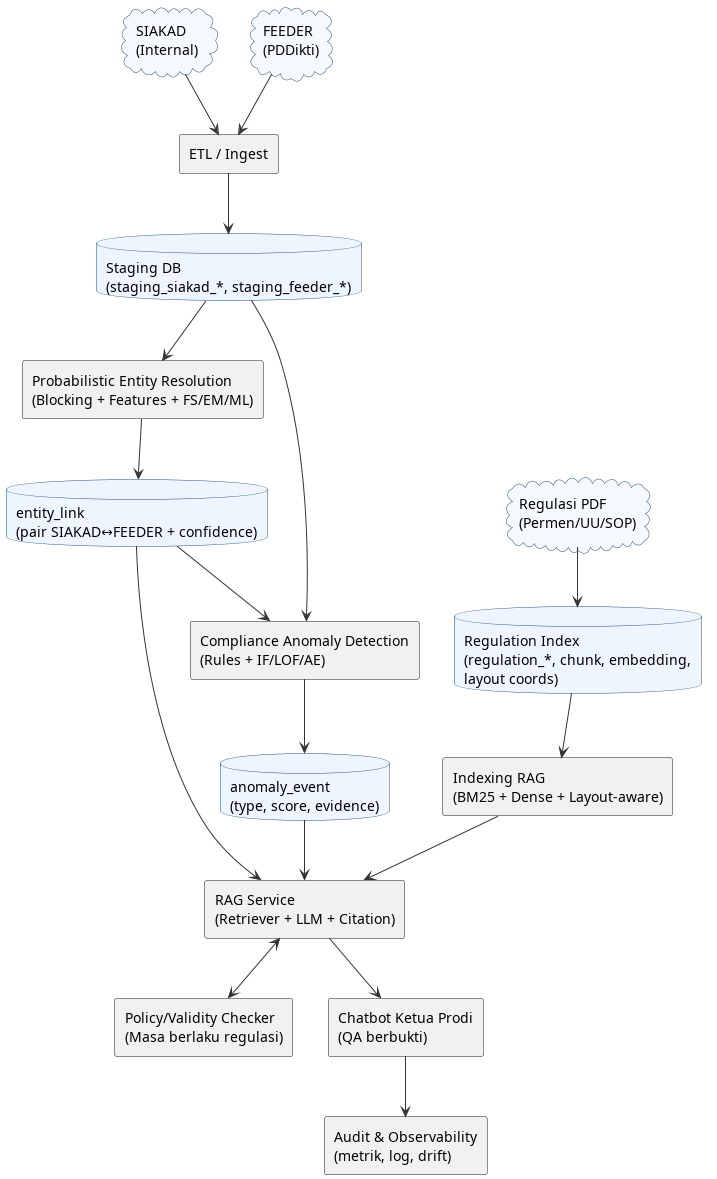
\includegraphics[width=0.7\linewidth]{DiagramKerangkaKonseptual.png}
                \caption{Diagram Kerangka Konseptual}
                \label{fig:kerangka}
            \end{figure}
    % ===================== HALAMAN BAB 4 (spasi 1.5) =====================
    \chapter{METODOLOGI PENELITIAN}
        \thispagestyle{empty}
        \section{Rencana Evaluasi}
    % ===================== DAFTAR PUSTAKA (spasi 1) =====================
    \printbibliography[title={Daftar Pustaka}]
\end{document}
